% !TEX root = ANA-GENR-2018-01-INT1.tex
% Turn off some chktex warnings.
% chktex-file 1 chktex-file 8 chktex-file 46

%------------------------------------------------------------------------------
\section{Analysis and paper phases}%
\label{sec:Analysis_and_paper_phases}
%------------------------------------------------------------------------------

For many years ATLAS used FENCE to support the approval process of Papers, CONF and PUB notes.
At that time, the three types of documents and their related interfaces were considered as independent systems.
They had different creation interfaces, different search interfaces and different workflows, all starting from \GSnote{Phase 1}{Phase 1 of what? LHC has a Phase I -- so this phrasing is confusing...}.
Recently, \GSnote{}{CERN has stopped supporting SVN...}since many projects at CERN changed their version control software from SVN~\cite{svn} to Git~\cite{gitlab}, the need of new FENCE system that could \GSnote{automatically create and configure GitLab repositories}{replace with ``interface with Git''} emerged.
Thus, the \GSnote{Analysis}{.. is it software for an analysis?}/\GSnote{Phase 0 software}{First time Phase 0 is mentioned. What is it?} was developed. It was also the opportunity to provide an interface which deals with the \enquote{Analysis only} workflow before accessing the Paper, CONF or PUB note production process. \GSnote{}{I don't understand this sentence.}
In this section, the way in which the software tools, mainly the FENCE framework already introduced in the previous section, are used to achieve the Analysis/Phase 0 requirements is presented.
In \cref{fig:Glance_Papers_Phase0}, a screenshot of the main interface of the system is shown, where the user can have an overview of all the analysis basic data (on the left) and Phase 0 steps (on the right).
It is also possible to move forward the workflow triggering automatic messages that alert the responsible for the next step that they should perform an action in the system, giving them instructions.

\begin{figure}[htb]
  \centering
  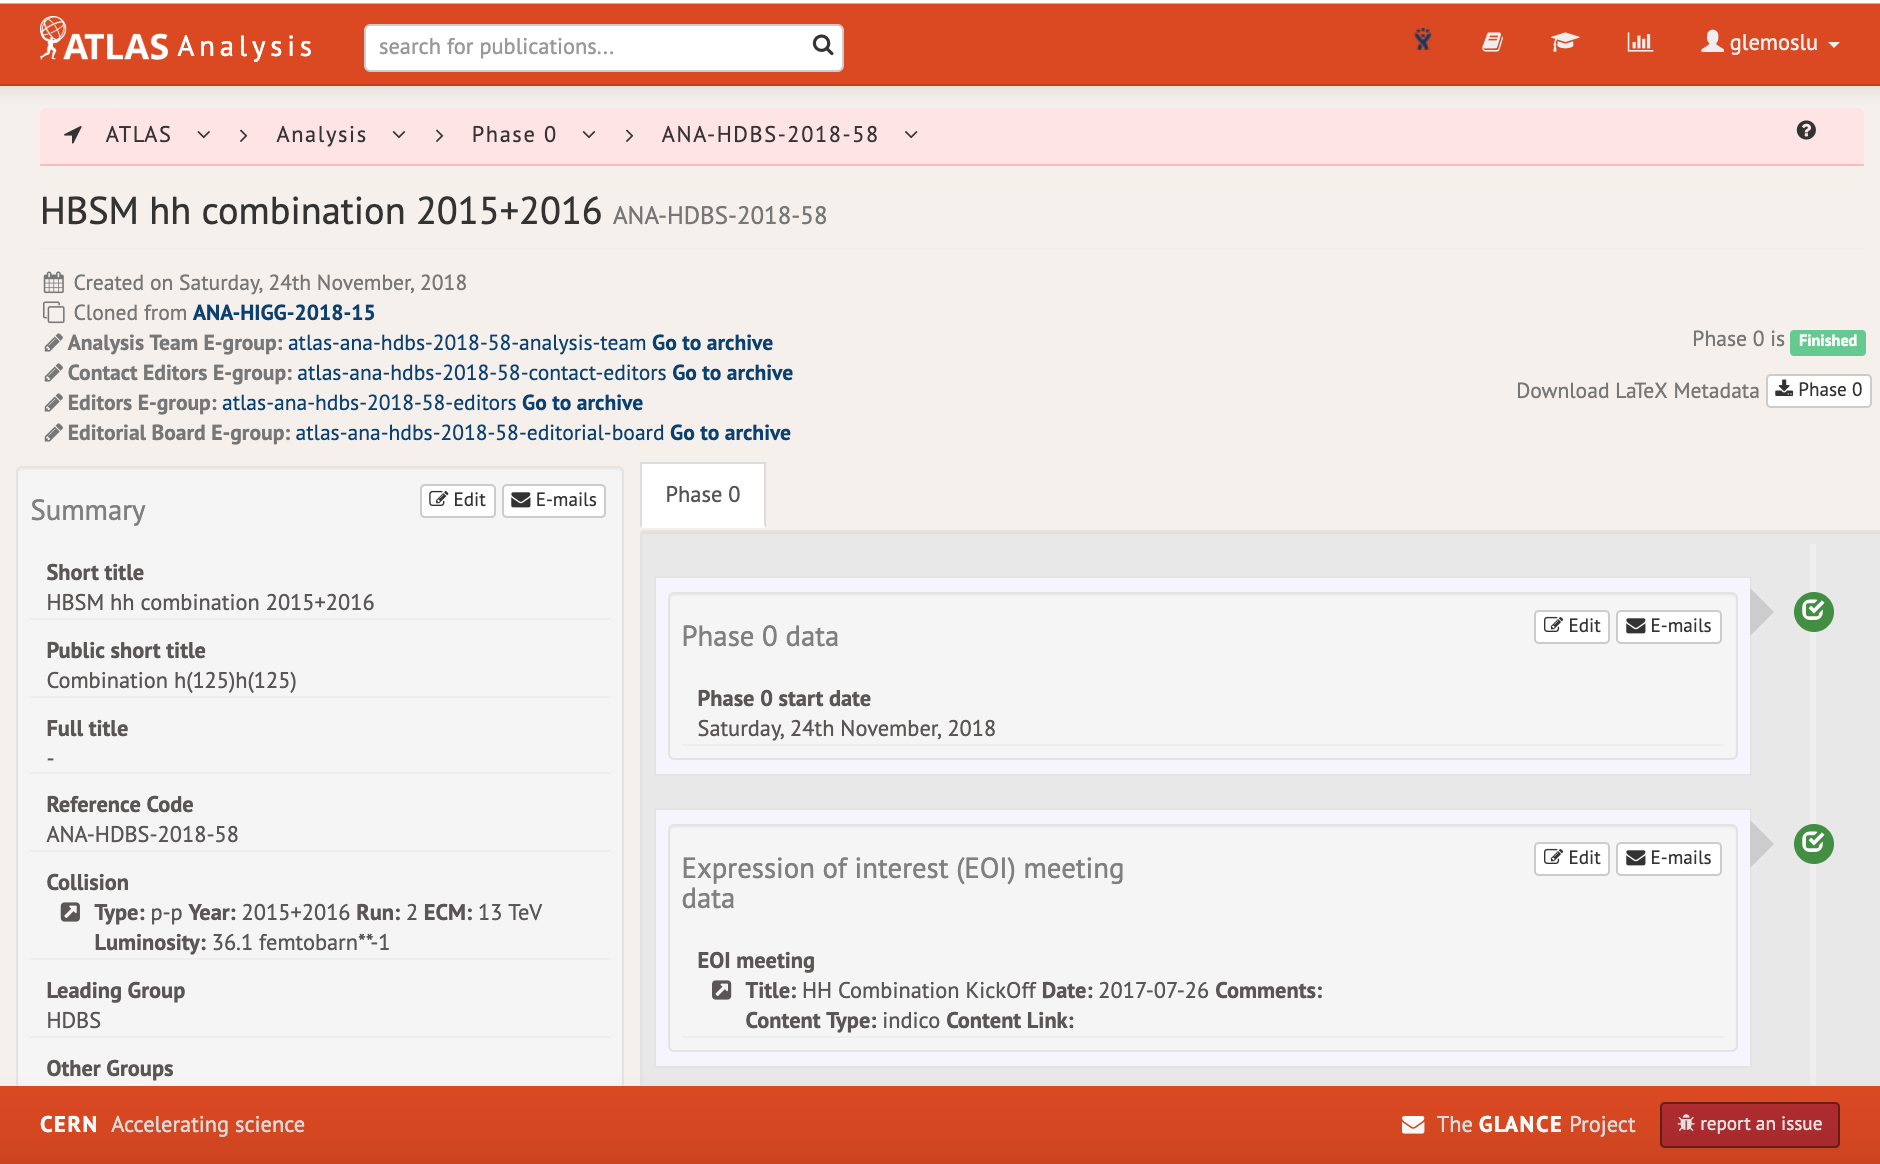
\includegraphics[width=0.9\textwidth]{figures/Glance_Papers_Phase0.png}
  \caption{Screenshot of the Analysis/Phase 0 system main interface. \GSnote{}{Expand this caption please. Mention what the reference code is, the name of the analysis, and what some of the data provided is.}}%
  \label{fig:Glance_Papers_Phase0}
\end{figure}

Phase 0 is a common stage for Papers, CONF and PUB notes workflows, before Phase 1.
It stores some metadata divided into steps, e.g.\ meeting dates, comments, links, groups of people like Analysis Contacts and the target date for analysis finalisation, Editorial board members and meetings, approval sign-off dates.
Each of those metadata should be filled in a \GSnote{specific order}{Is the order documented in this note?}, \GSnote{by certain users}{Is that documented in this note? Who?} and \GSnote{trigger automatic emails or egroups~\cite{egroups} updates}{Provide some examples of what kinds of emails or updates happen. Is it adding new people? Or creating new e-groups? With whom? etc...} along the process.
The main FENCE framework classes that allowed the development of those features are the \Class{Workflow}, \Class{Messenger}, \Class{EgroupManager} and \Class{User}.
Use is also made of many other classes and tools like the MBF (Models, Builder and Factories) infrastructure.
A brief explanation of the usage of each one is presented next.

%------------------------------------------------------------------------------
\subsection{\Class{Workflow} class}%
\label{sec:Workflow_class}

\GSnote{}{Is it a directed, acyclic graph (DAG)?}

The \Class{Workflow} class was developed based on the concept of Graphs, that encompasses the relation between objects. In this context, objects are called nodes and the relation between them are called edges, that can be a directional flow or not. To represent this concept through a codified depiction, some classes were created.

The abstract \Class{Graph} class, whose code can be found in \cref{sec:app1}, has a few simple implemented methods that allow the addition and deletion of nodes and edges.
The class that implements \Class{Graph} is called \Class{MapperGraph} and it stores nodes and edges inside a PHP data structure called \Structure{PSplObjectStorage}, that, for this implementation, could better manage objects than associative arrays.
The usage of this data structure allowed the development of very simple methods to retrieve neighbour nodes or even edges given its origin and target node, which means retrieving a directional edge.

The \Class{Node} class defines methods to set and get data related to one node. The Edge class defines similar methods, but related to an edge. An example of data that can be added to an edge is an instance of the \Class{Action} class, having methods to set and get function callbacks, defining its arguments and being able to access its outputs.
More details about the \Class{Action} class implementation can be found in \cref{sec:app2}.

The \Class{Workflow} class, one of the most important classes of the Analysis/Phase 0 system since it is mainly characterised with Phase 0 steps with actions in between them, uses the Graph, Node, Edge and Action classes. It defines nodes as being Phase 0 steps, edges as being the relation between them and having actions being triggered, for example, sending automatic emails, updating egroups~\cite{egroups} and saving data in the Database.

The behaviour of the \Class{Workflow} class is controlled by a JSON file, following the FENCE pattern described in \cref{sec:Configuration_files_in_FENCE}.
This file defines all Phase 0 steps, having their identifiers and the inputs that should be rendered in each step, specifying their types, rules and permissions.
It also has the actions that can be triggered from one step with their function callback and the next state which the workflow should be moved to. An example is shown in \cref{sec:app3}.

The \GSnote{example}{Show an except of that JSON file here? Don't just tell, also show!} is a part of the JSON file setting the step for analysis definition
after the Expression of Interest (EOI) meeting.
First, the identifier of the step is set as analysis$\_$definition.
Then, the main physics aim input is defined with its label, identifier, instructions (if any), type (in this case, a text box), its rule of maximum 500 characters and also the editor permissions. After, the actions are defined with their function callback path and permissions.
The callback can instantiate any other class like \Class{Messenger}, to send automatic emails or \Class{EgroupManager} to update egroups.
Finally, \GSnote{notifications to be sent}{What kind? Push notifications? Text? Email? Pigeon?} are defined through templates and specifying when they will be triggered.

%------------------------------------------------------------------------------
\subsection{Messenger class}%
\label{sec:Messenger_class}

The \Class{Messenger} class is used by the \Class{Workflow} class to send automatic emails and also to allow users to edit email templates. As explained before, the JSON file used by the \Class{Workflow} class defines email template names to be triggered by an action.
These templates and their variables are stored in the database in two JSON files.
The first one contains all the templates with variables to be substituted and the second contains the variables' identifiers and the methods used to substitute them in the templates before sending the email.
Using another class called \Class{DBJReader}, the \Class{Messenger} class can read these JSON files from the database.
Then, it can either get the templates and show them in the interface so the users can edit them or parse the variables and send an email.
In the first case, the changes performed in the templates are saved again in the database, but this time using the \Class{DBJWriter} class.
In the second case, \Class{Messenger} class will substitute all the variables in the template and use the \Class{Mailer} class to trigger the email to the correct recipient.
A summary of this infrastructure can be found in \cref{fig:Messenger_class}.

\begin{figure}[htb]
  \centering
  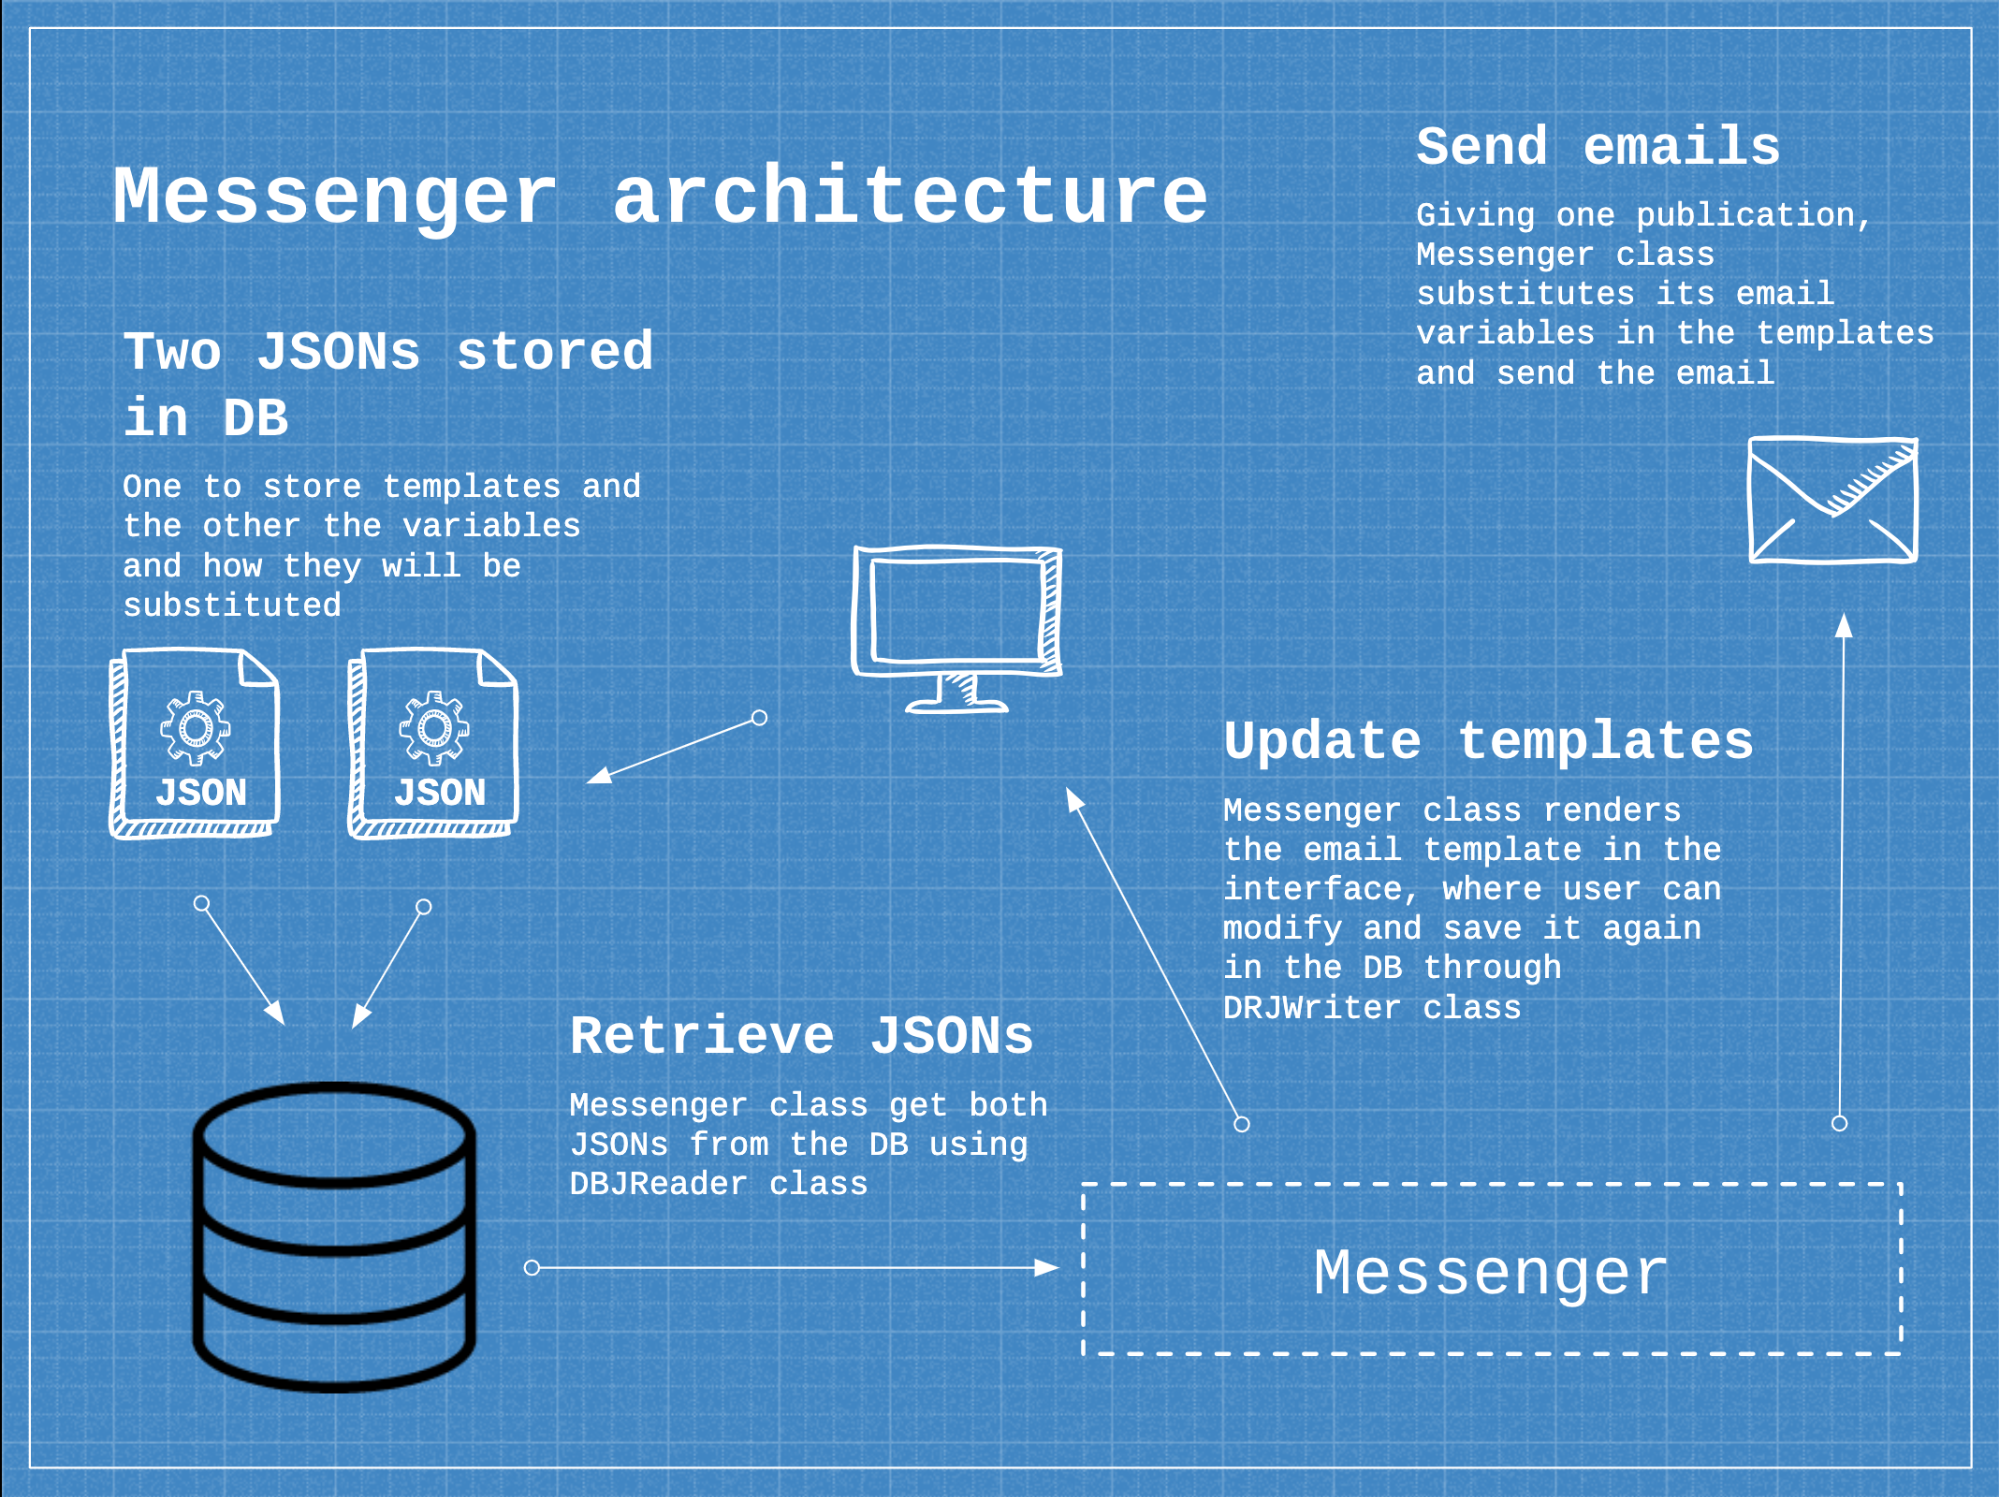
\includegraphics[width=0.9\textwidth]{Messenger_class}
  \caption{Summary of the \Class{Messenger} class infrastructure. \GSnote{}{Use this caption to explain the entire workflow depicte d in the diagram. Where am I looking at first? What's the order in which things happen? What's the computer icon in the middle? A user?}}%
  \label{fig:Messenger_class}
\end{figure}

In \cref{fig:email_template_editing} the interface that allows the editing and re-sending of an email template in shown. It is possible to set the recipients (To, CC and BCC), an additional email address not in the default list, the subject and the content of the email.
Those last two can have variables to be substituted according to the publication.

\begin{figure}[htb]
  \centering
  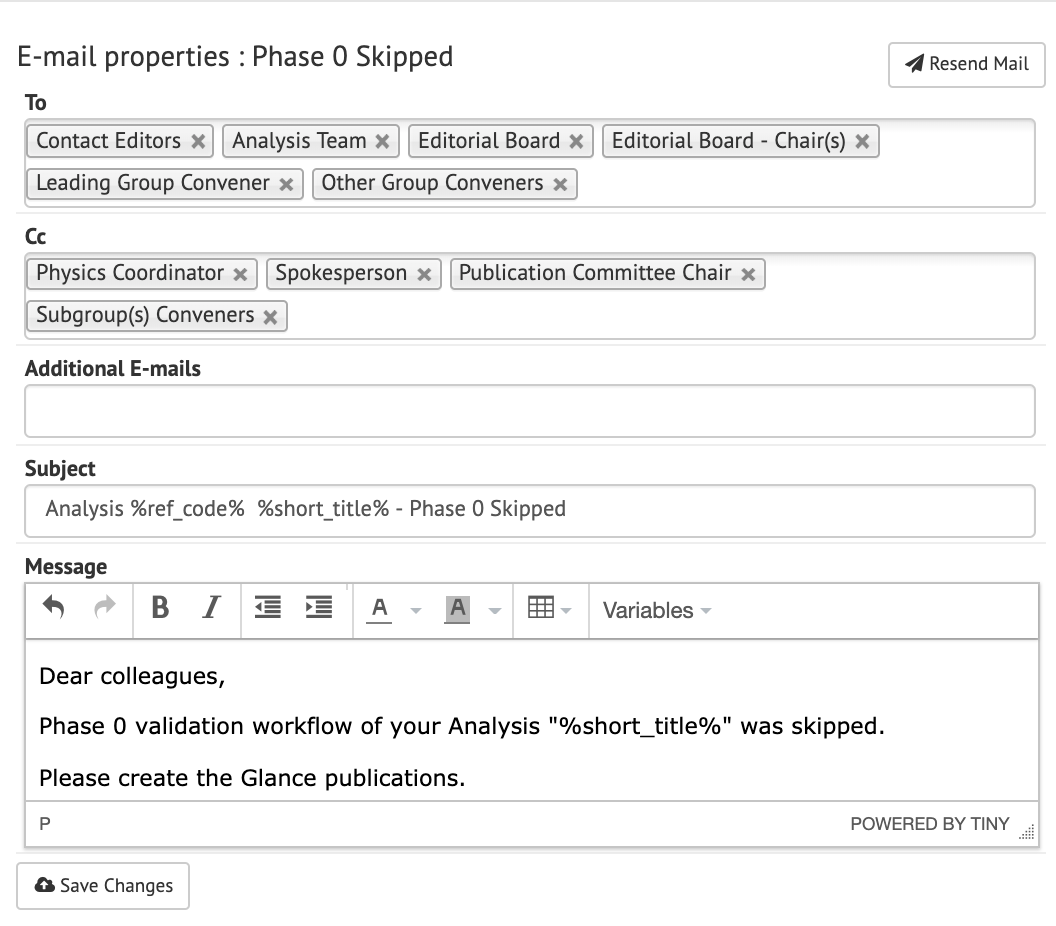
\includegraphics[width=0.9\textwidth]{email_template_editing}
  \caption{Interface for email template editing.}%
  \label{fig:email_template_editing}
\end{figure}


%------------------------------------------------------------------------------
\subsection{\Class{EgroupManager} class}%
\label{sec:EgroupManager_class}

The \Class{EgroupManager} class is similar to the \Class{Messenger} class since it also gets a template from a JSON file and substitutes variables.
The difference is that the templates are not related to email, but egroup configurations.
Also, it does not allow users to edit the templates from the interface since they contain many technical details used by the egroups API, explained \GSnote{later in this section}{add a ref please}.

The \Class{EgroupManager} class first uses another FENCE class to get the templates from the JSON file called \File{JReader}, designed to parse JSON files and save them in an object.
After getting the JSON templates, \Class{EgroupManager} parses it substituting all the variables.

One example that can be found in \cref{sec:app4} is the Analysis Team egroup created when there is a new Analysis/Phase 0 entry.
The template contains its identification, the name of the egroup with already one variable to be substituted, the Analysis/Phase 0 reference code.
It also defines a topic, administrator egroup and posting exceptions, some mandatory parameters to create an egroup through its API\@.
The members of the egroup will then be substituted by the Analysis team members when the \Class{EgroupManager} class parses the variables.

Having the template parsed, the \Class{EgroupManager} class uses the FENCE \Class{EgroupSOAPHandler} class to communicate with the egroups API\@.
To do so, it first makes an authentication and, using the methods available in the SOAP WebServices~\cite{egroups}, it can create, update or delete egroups.


%------------------------------------------------------------------------------
\subsection{\Class{User} class}%
\label{sec:User_class}

The main purpose of the \Class{User} class is to define an object that stores information concerning the logged in CERN member, for instance, his or her CERN CCID, first and last name, egroups and others attributes. Besides that, it defines specific methods, to facilitate the access control among the interface.
In \cref{sec:app5}, we have two examples of the above mentioned methods. These are used to check user \GSnote{clearance}{authorization}: \Class{is$\_$expert()} checks if the user is member of \enquote{fence-developers} egroup, which is composed by the project developers. % chktex 36
The method \Class{Permission($\$$permission)} accepts a permission to be checked as an argument and verifies if it is among the user permissions inventory. % chktex 36
Moreover, when an extension of \Class{User} is created, extra methods are appended to \Class{User} to provide specific \textit{utils} for a context.
This way, every system has its own \Class{User} class extending the FENCE core \Class{User} class.
This is the case for \Class{Analysis}, which has many specific methods used to grant edit permissions and control users access.
Furthermore, \Class{Analysis} was implemented using the concept of configuration files, described in \cref{sec:Configuration_files_in_FENCE}.
These files provide multiple properties that set access control and edit permissions on Analysis systems. This is mainly achieved in two ways. General access control is set using CERN egroups, or FENCE user groups, such as experts, administrators and many others.
In this case, \Class{User} class verifies the clearance by comparing the user egroups and user groups to the ones contained on its object.
The other way concerns inputs edit permissions and uses analysis specific roles to do so.
These roles are keys mapped to methods in \Class{User} class that check if the member is supposed to have edit permission on that specific field.
\GSnote{An example is shown in \cref{sec:app6}}{Why can't we show the example here near the explanation?}.


%------------------------------------------------------------------------------
\subsection{MBF (Models, Builder and Factories) infrastructure}%
\label{sec:MBF_Models_Builder_and_Factories_infrastructure}

Models, Builders and Factories are all individually heavily used software design patterns.
However, their combined usage is a particular feature of FENCE framework.
The main goal of these development standards is to create a wrapper to store complex objects and facilitate the construction of these on different contexts.
For instance, it would be possible to pass an actual SQL Query every time information from the database is needed.
It is, however, much more convenient to just call a class that handles the queries and presents to the user the needed object.
The desired behaviour described above is exactly how the MBF infrastructure works. \GSnote{}{It might be cleaner to refer to this as a SQL query builder -- common phrase used in industry}
On FENCE classes, objects are constructed simply by instantiating specific factories classes.
These classes extend the core \Class{Factory} class, which sets the whole engineering that connects to the database and assembles objects.
Whenever a specific new object needs to be created, a group of three files are needed: the Factory, the Builder and the Model files.
Models are classes that serve as an oriented object representation of the information. They define several sets and get methods that handle specific properties of the object. These models are used in Builders, where the actual query is set and database columns are associated to a model set method. Finally, a Factory calls its corresponding Builder and also contains an inventory, which may be empty, of other Factories that are related to this object.

The \Class{Workflow}, \Class{Messenger}, \Class{EgroupManager} and \Class{User} classes, along with the MBF infrastructure made possible the development of the Analysis/Phase 0 system workflow, well represented by \cref{fig:Glance_Papers_Phase0}.
However, they do not include the GitLab Integration, a key feature of the system, that will be explained in detail in the next sections.

\GSnote{}{More example code, and charts/trees would help to clarify a lot of this. There's a lot of text that's very dense and hard to parse without more figures.}
